\documentclass{article}
\usepackage{iclr2022_conference,times}
\usepackage{amsmath,amssymb}
\usepackage{graphicx}
\usepackage{booktabs}
\usepackage{listings}
\usepackage{xcolor}
\usepackage[utf8]{inputenc}
\usepackage{url}
\usepackage{caption}

\captionsetup{font=footnotesize,labelfont=bf,skip=2pt}
\setcounter{topnumber}{2}
\renewcommand{\topfraction}{0.92}
\renewcommand{\textfraction}{0.05}
\renewcommand{\floatpagefraction}{0.75}
\setlength{\textfloatsep}{4pt}
\setlength{\intextsep}{4pt}
\setlength{\abovecaptionskip}{2pt}
\setlength{\belowcaptionskip}{0pt}

\definecolor{codebg}{HTML}{F5F5F2}
\definecolor{codemuted}{HTML}{898781}
\lstset{
  basicstyle=\ttfamily\scriptsize,
  backgroundcolor=\color{codebg},
  commentstyle=\color{codemuted},
  frame=single, rulecolor=\color{codemuted}, framesep=2pt,
  xleftmargin=4pt, aboveskip=2pt, belowskip=2pt,
  breaklines=true, columns=fullflexible, showstringspaces=false,
}

\title{CodeLangID: A Character-Level CNN for\\Programming Language Identification}

\author{Mohamad Salman \;\textbar\; \texttt{mohamad.salman@mail.utoronto.ca} \;\textbar\;
University of Toronto \;\textbar\; \textbf{Solo project} \\
Code: \url{https://github.com/mohamadmsalman82/codelangid}}

\iclrfinalcopy

\begin{document}
\maketitle
\lhead{APS360: Applied Fundamentals of Deep Learning --- Project Progress Report}
\thispagestyle{fancy}

\vspace{-18pt}
\section{Brief Project Description}
\vspace{-4pt}

Syntax highlighters, code search engines, snippet managers and Q\&A sites such as Stack
Overflow must constantly identify a block of code's language, often from a short,
context-free fragment with no filename or extension \citep{alreshedy2018scc}.
\textbf{This project maps a raw snippet to one of 10 popular languages (Python, Java,
C++, JavaScript, Go, C, Ruby, PHP, Rust, C\#) from its characters alone.} Extensions and
editor metadata are exactly what is missing in pasted snippets, chat messages and scraped
pages, and rule-based detectors degrade on short or ambiguous fragments
\citep{vandam2016software}; GitHub's Linguist leans on extensions and heuristics
\citep{linguist}, so it says little about a bare snippet---the gap a learned model fills.

Deep learning fits for three reasons. Languages differ by \emph{subtle, overlapping} cues
(keywords, operator spellings, bracket and indentation patterns) that a character-level CNN
learns automatically rather than by hand-engineering features per language
\citep{zhang2015character}. Character input also side-steps a chicken-and-egg problem: a
token-based model needs a tokenizer, but choosing one presupposes knowing the language. And
the cues are \emph{local} n-gram motifs (\texttt{:=}, \texttt{\#include})---what
small-kernel convolution detects \citep{kim2014convolutional}. Figure~\ref{fig:pipeline}
gives the contract: \textbf{input} raw text padded/truncated to 256 characters,
\textbf{output} a softmax over the 10 languages.

\begin{figure}[h]
\centering
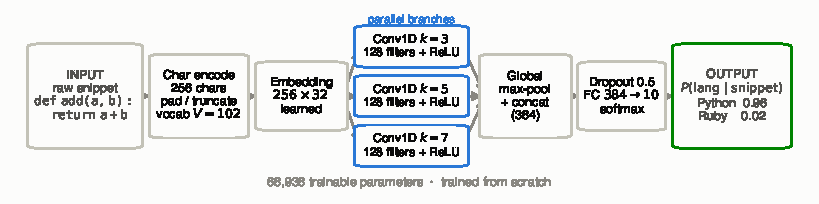
\includegraphics[width=\textwidth]{fig_pipeline.pdf}
\vspace{-5pt}
\caption{The CodeLangID pipeline. \textbf{Input}: a raw snippet, any language, encoded
character-by-character into a fixed 256-token window. \textbf{Output}:
$P(\mathrm{lang}\mid\mathrm{snippet})$ over the 10 classes.}
\label{fig:pipeline}
\end{figure}

\vspace{-12pt}
\section{Individual Contributions and Responsibilities}
\label{sec:contrib}
\vspace{-4pt}

This is a \textbf{solo project}: there are no other team members, so every item in
Table~\ref{tab:contrib} is my own work and I hold all responsibilities end to end. All
code is reproducible (\texttt{src/}, seed 360); every number below regenerates from a
clean checkout.

\begin{table}[h]
\centering\footnotesize
\caption{Work breakdown; all items are my sole responsibility (solo project). Final tuning
and the report remain in progress.}
\label{tab:contrib}
\vspace{-3pt}
\begin{tabular}{@{}llp{7.3cm}@{}}
\toprule
\textbf{Component} & \textbf{Status} & \textbf{Evidence / artefact} \\
\midrule
Data collection \& cleaning  & Complete & \texttt{build\_dataset.py}: 10{,}360 snippets (Table~\ref{tab:clean}) \\
Held-out test collection     & Complete & \texttt{scrape\_heldout.py}: 740 snippets, 24 repos, 0 leaked \\
Baseline model               & Complete & \texttt{baseline.py}: 90.14\% test (Table~\ref{tab:results}) \\
Primary model (char-CNN)     & Complete & \texttt{cnn.py}: 92.74\% test, 82.84\% held-out \\
Alternative model (BiGRU)    & Complete & \texttt{gru.py}: tried and \textbf{rejected} (\S\ref{sec:primary}) \\
Evaluation \& error analysis & Complete & \texttt{figures.py}: Fig.~\ref{fig:cm}, \S\ref{sec:qual} \\
\bottomrule
\end{tabular}
\vspace{-8pt}
\end{table}

\vspace{-4pt}
\section{Notable Contribution}
\vspace{-4pt}

My notable contribution is the \textbf{complete working pipeline}: a cleaned balanced
dataset, a classical baseline, a char-CNN that beats it, and an independently collected
held-out set exposing a diagnosable failure mode.

\vspace{-6pt}
\subsection{Data Processing}
\vspace{-4pt}
\textbf{Source.} Rosetta Code \citep{rosettacode} (\texttt{acmeism/RosettaCodeData}
mirror) implements the same tasks across many languages, so snippets are balanced and
labelled by directory structure rather than guessed. Table~\ref{tab:clean} gives the full
pipeline (\texttt{src/build\_dataset.py}, seed 360) and its yield, specified so a
classmate can reproduce it. Two steps carry most of the weight. \emph{Near-duplicate
removal}: Rosetta hosts many near-identical variants of one solution, so MinHash/LSH over
5-character shingles drops pairs with Jaccard $\geq0.8$ \citep{broder1997resemblance}.
\emph{Splitting by task, not by file}: all snippets from a task land in one split---else two
``Bubble sort'' solutions straddle train and test and inflate accuracy. Each snippet is
emitted in \textbf{two variants}, \texttt{raw} and \texttt{nocomment}, to test reliance on
comment prose versus code structure.

\begin{table}[h]
\centering\footnotesize
\caption{Cleaning pipeline and yield (steps 2--4 run during windowing, so the running total
is first well-defined at step 4). Result: 10{,}360 snippets, 1{,}036 per class (chance
$=$ 10\%), split 1{,}162/249/250 \emph{tasks}.}
\label{tab:clean}
\vspace{-3pt}
\begin{tabular}{@{}rlrr@{}}
\toprule
\textbf{\#} & \textbf{Operation} & \textbf{Removed} & \textbf{Remaining} \\
\midrule
1 & Read 10 language directories & --- & 18{,}654 files \\
2 & Window: $\leq$3 line-aligned 256-char windows/file ($\geq$3 lines, $\geq$64 char) & 1{,}125 files & \\
3 & Comment/markup filter: drop if comments $>$50\% of non-space chars & 3{,}460 win. & \\
4 & Exact dedup: SHA-1 of whitespace-normalized text & 327 win. & 38{,}394 snippets \\
5 & Near-dup dedup: MinHash (64 perm, 16 LSH bands), Jaccard $\geq0.8$ & 353 & 38{,}041 \\
6 & Balance: cap each class at 1{,}036 $=$ smallest class (PHP) & 27{,}681 & \textbf{10{,}360} \\
7 & Split \emph{by task} 70/15/15 (no task spans two splits) & --- & 7{,}225 / 1{,}634 / 1{,}501 \\
8 & Encode: vocab $V{=}102$ (ASCII\,$+$\,\texttt{<pad>}\,$+$\,\texttt{<unk>}), pad/truncate to 256 & --- & --- \\
\bottomrule
\end{tabular}
\vspace{-6pt}
\end{table}

\textbf{Example cleaned training sample} (class \textsc{Python}, 173 characters):
\begin{lstlisting}[language=Python]
def mkdirp(path):
    try: os.makedirs(path)
    except OSError as exc: # Python >2.5  <- removed in the `nocomment' variant
        if exc.errno == errno.EEXIST and os.path.isdir(path): pass
        else: raise
\end{lstlisting}

\textbf{Plan for never-before-seen data.} Rather than reuse a public dataset I collected the
final test set myself (\texttt{src/scrape\_heldout.py}): \textbf{740 snippets from 24 real
GitHub repositories} (e.g.\ \texttt{psf/requests}, \texttt{redis/redis},
\texttt{BurntSushi/ripgrep}), 74 per language, through the \emph{identical} pipeline. None is
a Rosetta source, and it is deliberately a \emph{different distribution}: production library
code, not puzzle solutions. Each snippet is checked against the SHA-1 of every training
snippet---\textbf{0 leaked}---and is never trained or tuned on.

\textbf{Challenges.} (i) PHP is thin on Rosetta (645 usable files vs.\ Python's 3{,}054), so
balancing drags \emph{every} class to 1{,}036---the biggest limit on dataset size.
(ii) Splitting by snippet leaked near-identical solutions and inflated early accuracy;
splitting by task fixed it. (iii) The regex comment stripper over-strips string literals
containing \texttt{//} or \texttt{\#}; acceptable as it is applied uniformly.

\vspace{-6pt}
\subsection{Baseline Model}
\vspace{-4pt}

The baseline uses no deep learning: TF-IDF over \textbf{character n-grams}
($n\!\in\![1,3]$, \texttt{min\_df}=2, sublinear tf, case preserved) into \textbf{Multinomial
Naive Bayes} on the same splits, mirroring prior work
\citep{khasnabish2014detecting,ugurel2002whats}. It needs no tuning beyond the fixed n-gram
range, uses 43{,}573 features and trains in $\approx$4\,s. It is an honest bar, not a straw
man---\textbf{90.14\%} versus 10\% chance---so n-grams already carry most of the signal and
the CNN must justify itself on what remains.

\vspace{-6pt}
\subsection{Primary Model}
\label{sec:primary}
\vspace{-4pt}

The primary model (Figure~\ref{fig:pipeline}) is \texttt{Embedding}$(102,32)$
(\texttt{padding\_idx}=0); three \emph{parallel} \texttt{Conv1d} branches of widths 3/5/7,
128 filters each $+$ ReLU; global max-pool per branch; concatenation to 384;
\texttt{Dropout}(0.5); \texttt{Linear}$(384,10)$ $+$ softmax. Parallel widths rather than a
deep stack see 3-, 5- and 7-character motifs at once---the scale at which
\texttt{fn}, \texttt{:=} and \texttt{\#include} live. It has \textbf{68,938 trainable
parameters} in 5 weight layers, trained from scratch with cross-entropy and Adam
\citep{kingma2015adam} (lr $10^{-3}$, batch 64, $\leq$30 epochs, early stopping on
validation accuracy, patience 6). Training takes \textbf{35\,s} on an Apple M-series GPU
(MPS). Validation loss flattens near epoch 10 and the train/validation gap widens after
epoch 12---mild overfitting that early stopping controls: it stopped at epoch 25 with
the best validation accuracy at \textbf{epoch 19}.

I also built the proposal's bidirectional GRU (\texttt{src/gru.py}; embedding 32, hidden
64/direction, max-pooled, 42{,}186 parameters). \textbf{It did not pan out}---the most
useful negative result so far: 90.27\% test, indistinguishable from Naive Bayes and 2.5
points below the CNN, while taking \textbf{647\,s to train, 18$\times$ the CNN}. Language
identity in a 256-character window rests on \emph{local} motifs, so recurrence buys
nothing and costs much; the CNN stays primary.

\begin{figure}[t]
\centering
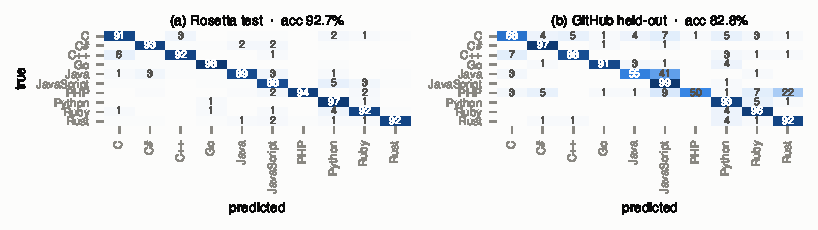
\includegraphics[width=\textwidth]{fig_confusion.pdf}
\vspace{-11pt}
\caption{Char-CNN confusion, row-normalized (cell $=$ \% of the true class predicted as
that column). (a) Rosetta test. (b) Never-before-seen GitHub held-out, where
Java$\to$JavaScript and PHP$\to$Rust dominate (\S\ref{sec:qual}).}
\label{fig:cm}
\end{figure}

\vspace{-8pt}
\subsection{Quantitative and Qualitative Results}
\label{sec:qual}
\vspace{-4pt}

\textbf{Quantitative.} The char-CNN wins on every split (Table~\ref{tab:results}):
\textbf{92.74\%} (macro-F1 0.927, cross-entropy 0.238) on the Rosetta test split,
\textbf{+2.60} over the baseline, and \textbf{82.84\%} (macro-F1 0.822, loss 0.495) on
the never-before-seen GitHub set, \textbf{+3.25} over it.

\begin{table}[h]
\centering\footnotesize
\caption{All models, both test sets (accuracy \%). ``Held-out'' $=$ never-before-seen
GitHub data. Chance 10\%. Best in bold.}
\label{tab:results}
\vspace{-3pt}
\begin{tabular}{@{}llrrrr@{}}
\toprule
\textbf{Model} & \textbf{Variant} & \textbf{Params} & \textbf{Val} &
\textbf{Test (Rosetta)} & \textbf{Held-out (GitHub)} \\
\midrule
TF-IDF + NB (baseline)      & raw       & 43{,}573\,ft & 91.80 & 90.14 & 79.59 \\
TF-IDF + NB (baseline)      & nocomment & 41{,}472\,ft & 91.48 & 89.27 & 81.89 \\
Char-BiGRU (rejected)       & raw       & 42{,}186 & 92.59 & 90.27 & 80.54 \\
\textbf{Char-CNN (primary)} & raw       & 68{,}938 & \textbf{94.31} & \textbf{92.74} & \textbf{82.84} \\
\textbf{Char-CNN (primary)} & nocomment & 68{,}938 & 94.69 & 92.49 & 82.16 \\
\bottomrule
\end{tabular}
\vspace{-4pt}
\end{table}

\textbf{Comment ablation.} Stripping comments costs the CNN only \textbf{0.25} points
(92.74$\to$92.49): it reads \emph{code structure, not comment prose}---what the two variants
were built to test. The baseline behaves oppositely---removing comments \emph{improves} its
held-out score by 2.30 points (79.59$\to$81.89)---so comment text misleads a bag-of-n-grams
model on real code while the CNN is largely immune.

\textbf{Qualitative.} The 9.9-point gap between the two test sets (Figure~\ref{fig:cm})
is the most interesting result so far, because the errors explain it. Two non-random modes
dominate. \emph{(1) Java$\to$JavaScript (30 errors): licence headers.} \textbf{22 of the
30} contain an Apache/copyright header, and on average only \textbf{17\% of their
non-whitespace characters are code}---the rest is English prose in a \texttt{/*~*/} block.
Rosetta files carry no licence headers, so the model never learned that a real file's first
256 characters are often boilerplate identical across languages; it is starved of code, not
wrong. \emph{(2) PHP$\to$Rust (16 errors): PHP 8 attributes.} \textbf{13 of the
16} contain \texttt{\#[}, diagnosable straight from the training data: \texttt{\#[} occurs
in \textbf{0.0\% of PHP training snippets (0/753)} but \textbf{9.0\% of Rust (63/703)}, so
the model learned the rule \texttt{\#[}$\Rightarrow$Rust. PHP 8 spells attributes identically
(\texttt{\#[Group('...')]}) and they appear in \textbf{18.9\% of held-out PHP (14/74)}, but
Rosetta's PHP predates PHP 8 so the construct is invisible in training. This is textbook
\emph{distribution shift}---confidently wrong for a legible reason---and PHP's F1 collapses
from 0.97 in-distribution to 0.66 held-out.

\textbf{Challenges.} (i) The held-out set took the most work: my first version yielded only
34 snippets/class because the C repositories I picked were too small, so I widened the
list. (ii) The BiGRU's 18$\times$ training cost made hyperparameter search impractical.
(iii) MPS lacks deterministic kernels, so results move $\approx\pm0.3$ points at a fixed
seed; I treat sub-0.5-point gaps as noise. \textbf{On feasibility}\label{sec:feas}: all data
is obtained, the baseline is beaten on both test sets, and the pipeline reruns in under 3
minutes, so the work the error analysis points to---licence-header stripping (mode 1),
post-2015 PHP sources (mode 2), and SCC \citep{alreshedy2018scc}---is comfortably achievable
by the final report.

\bibliographystyle{iclr2022_conference}
\bibliography{refs}

\end{document}
